\chapter{UJI COBA DAN EVALUASI}
Pada bab ini akan dijelaskan tentang uji coba dan evaluasi dari implementasi sistem yang telah dilakukan pada bab 4.

\section{Lingkungan Uji Coba}
Lingkungan uji coba menggunakan sebuah komputer dengan spesifikasi perangkat keras dan perangkat lunak sebagai berikut.

\begin{enumerate}
	\item Perangkat Keras
	\begin{enumerate}
		\item GPU: 1x Tesla K80 , having 2496 CUDA cores, compute 3.7, 12GB(11.439GB Usable) GDDR5 VRAM.
		\item CPU: 1x single core hyper threaded i.e(1 core, 2 threads) Xeon Processors @2.3Ghz (No Turbo Boost) , 45 MB Cache.
	\end{enumerate}
	\item Perangkat Lunak
	\begin{enumerate}
		\item Sistem Operasi Linux Ubuntu 1804 64-bit
		\item Android Studio
		\item Bahasa Pemrograman Java
		\item Bahasa Pemrograman Python
		\item Library Keras
	\end{enumerate}
\end{enumerate}

\section{Dataset}
\par Dataset yang digunakan adalah dataset daun dari \url{https://archive.ics.uci.edu/ml/datasets/leaf}. Dataset ditambahkan dengan dataset dari penulis sendiri. Dataset akan dipecah dengan rasio 7 : 3 untuk data train dan data test. 

\section{Uji Coba Ekstraksi Fitur Menggunakan Pre-Trained Model}

\par Hasil dari evaluasi pembuatan model yang diekstraksi dengan \textit{pre-trained model} yang disediakan adalah :


\begin{table}[ht]
	\centering
	\begin{tabularx}{1.0\textwidth}
		{|p{2cm}|X|X|X|X|}
	\hline
	\rowcolor{lightgray} \centering Model&Rank-1&Precision&Recall&F1 Score \\ \hline
	\centering VGG16	& 	95.62 & 	97.0	& 96.0	&	95.0 \\ \hline
	\centering VGG19	& 94.89 &	96.0	&95.0	& 94.0 \\ \hline
    \rowcolor{green} \centering MobileNet	&	96.35	& 97.0	& 96.0 &	96.0 \\ \hline
	\centering ResNet50	& 53.28	& 61.0	& 53.0	& 51.0 \\ \hline
	\centering InceptionV3	&	93.43	&  95.0 & 93.0 & 93.0 \\ \hline
	\centering Xception	&	93.43	& 95.0 & 93.0 & 93.0 \\ \hline
	\end{tabularx}
	\caption{Tabel data hasil evaluasi model}
	\label{table:hasil}
\end{table}

\begin{table}[ht]
	\centering
	\begin{tabularx}{1.0\textwidth}
		{|X|X|}
		\hline
		\rowcolor{lightgray} \centering Model& Waktu Ekstraksi Fitur \\ \hline
		\centering VGG16	& 	8 menit 56 detik \\ \hline
		\centering VGG19	& 10 menit 3 detik \\ \hline
		\rowcolor{green} \centering MobileNet	&	2 menit 5 detik \\ \hline
		\centering ResNet50	& 15 menit 27 detik	\\ \hline
		\centering InceptionV3	&	6 menit \\ \hline
		\centering Xception	&	5 menit 38 detik \\ \hline
	\end{tabularx}
	\caption{Tabel data waktu ekstraksi fitur}
	\label{table:hasil}
\end{table}

Dari hasil tersebut, dapat disimpulkan bahwa arsitektur yang optimal dalam pengklasifikasian jenis daun adalah MobileNet. MobileNet memiliki akurasi paling tinggi, 96.35\% dan waktu ekstraksi fitur paling cepat yaitu 2 menit 5 detik.

\section{Hasil dari Aplikasi}
Berikut adalah hasil tangkapan layar dari aplikasi :

\begin{figure}[ht]
\begin{subfigure}{0.5\textwidth}
	\centering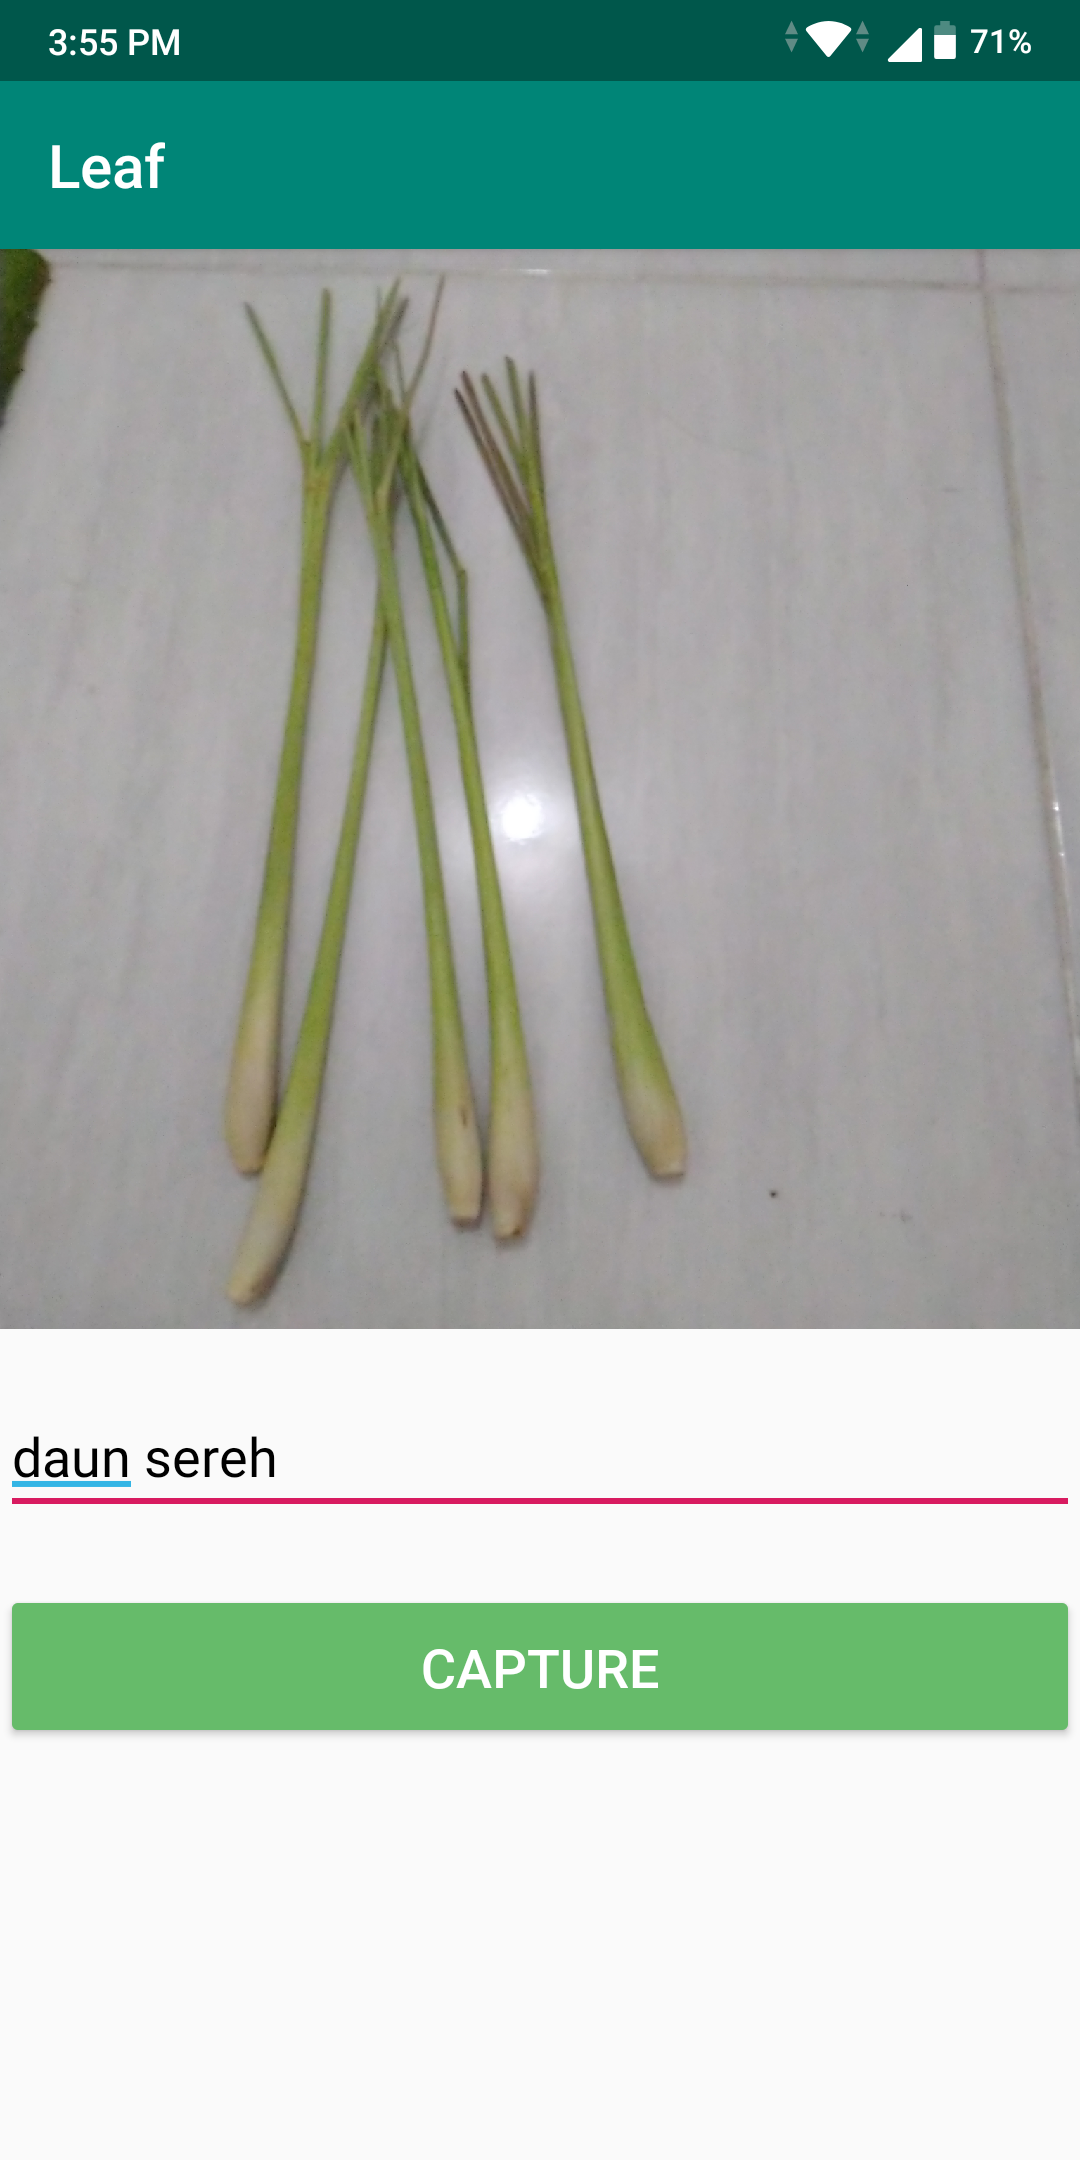
\includegraphics[width=\linewidth]{bab5/figures/uploadsereh.png}
	\caption{Fungsi Upload}
	\label{fig:analisis_label_a}
\end{subfigure}
~
\begin{subfigure}{0.5\textwidth}
	\centering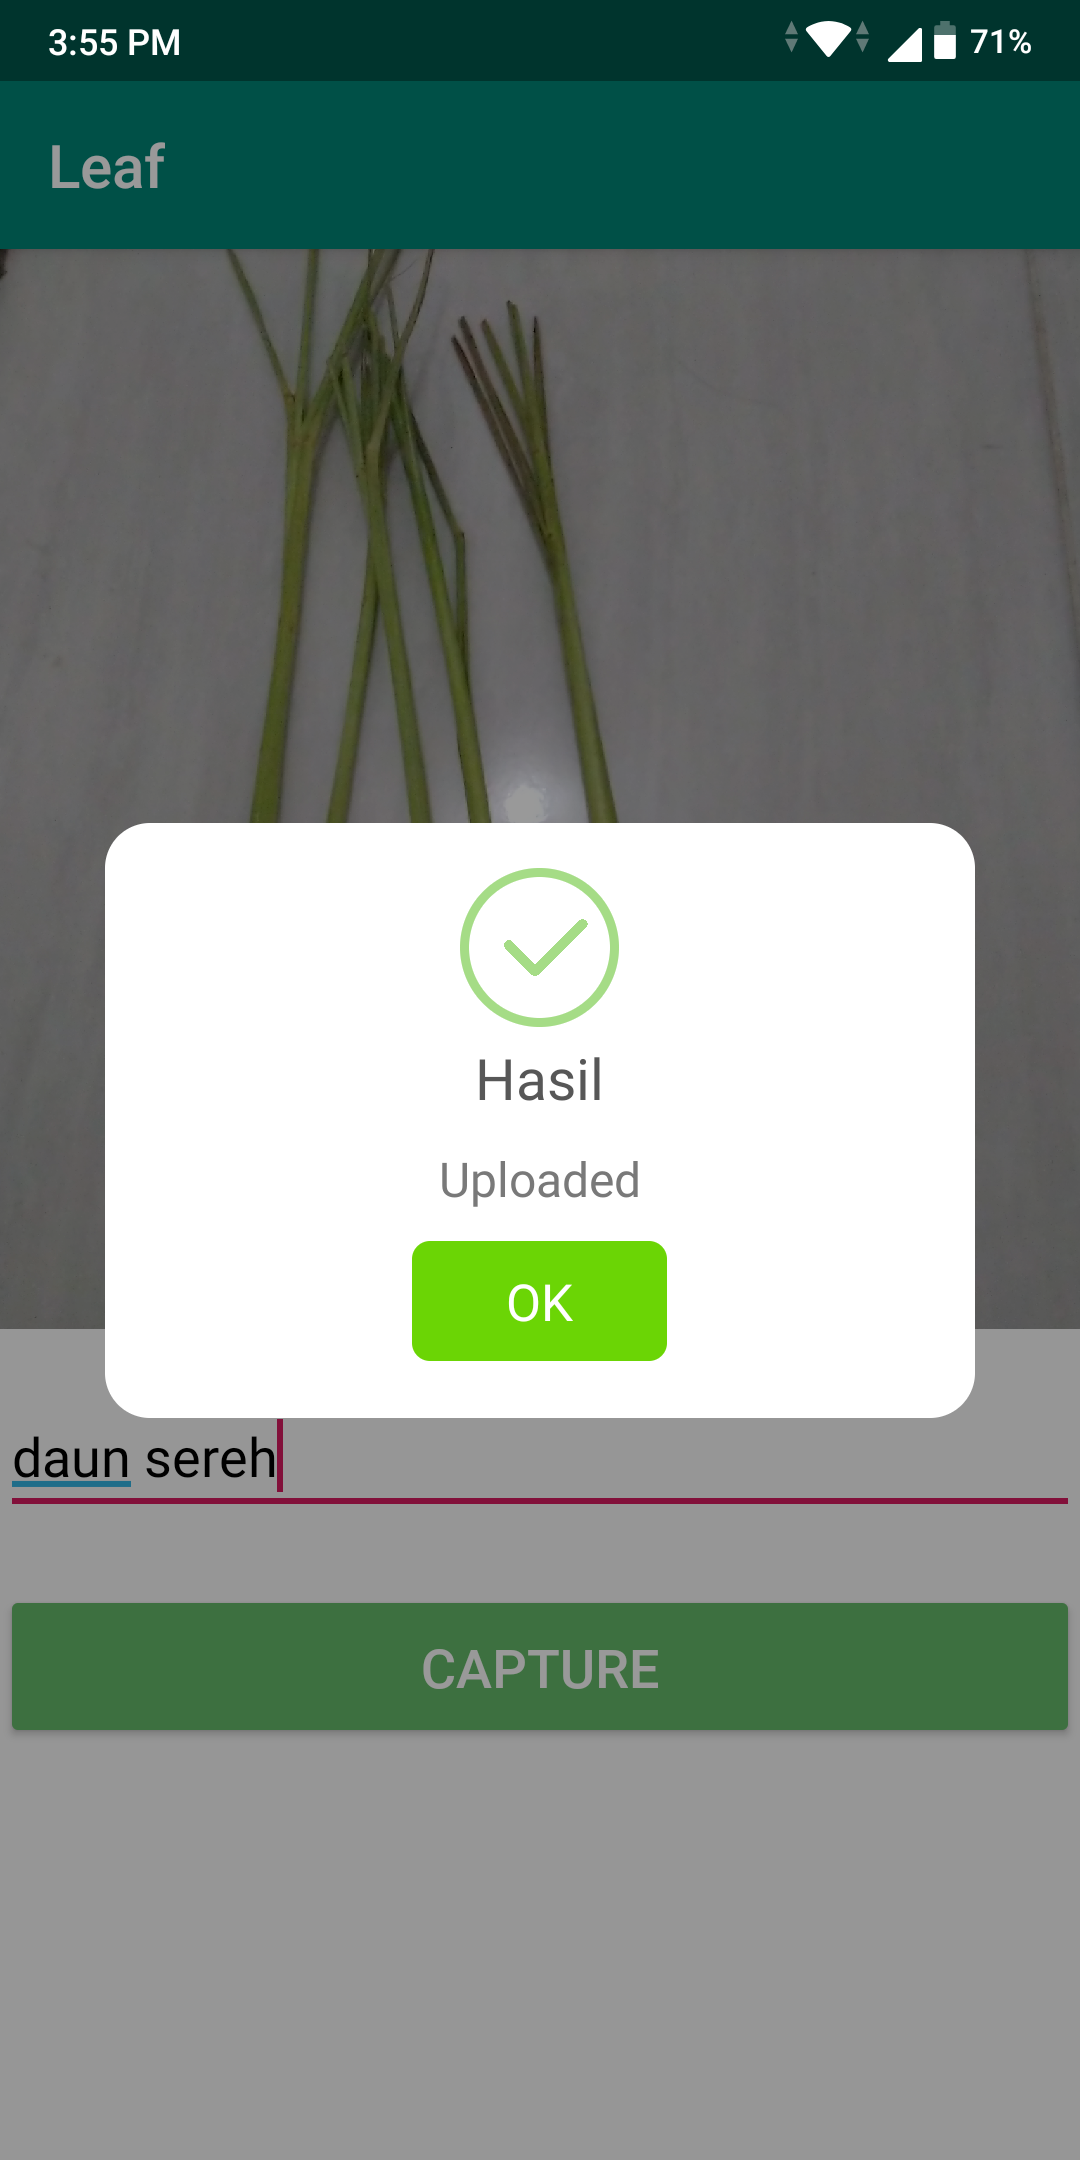
\includegraphics[width=\linewidth]{bab5/figures/uploaded.png}
	\caption{Berhasil Upload}
	\label{fig:analisis_label_b}
\end{subfigure}
\caption{Hasil tangkap layar pada fitur Upload}
\end{figure}

\begin{figure}[ht]
	\centering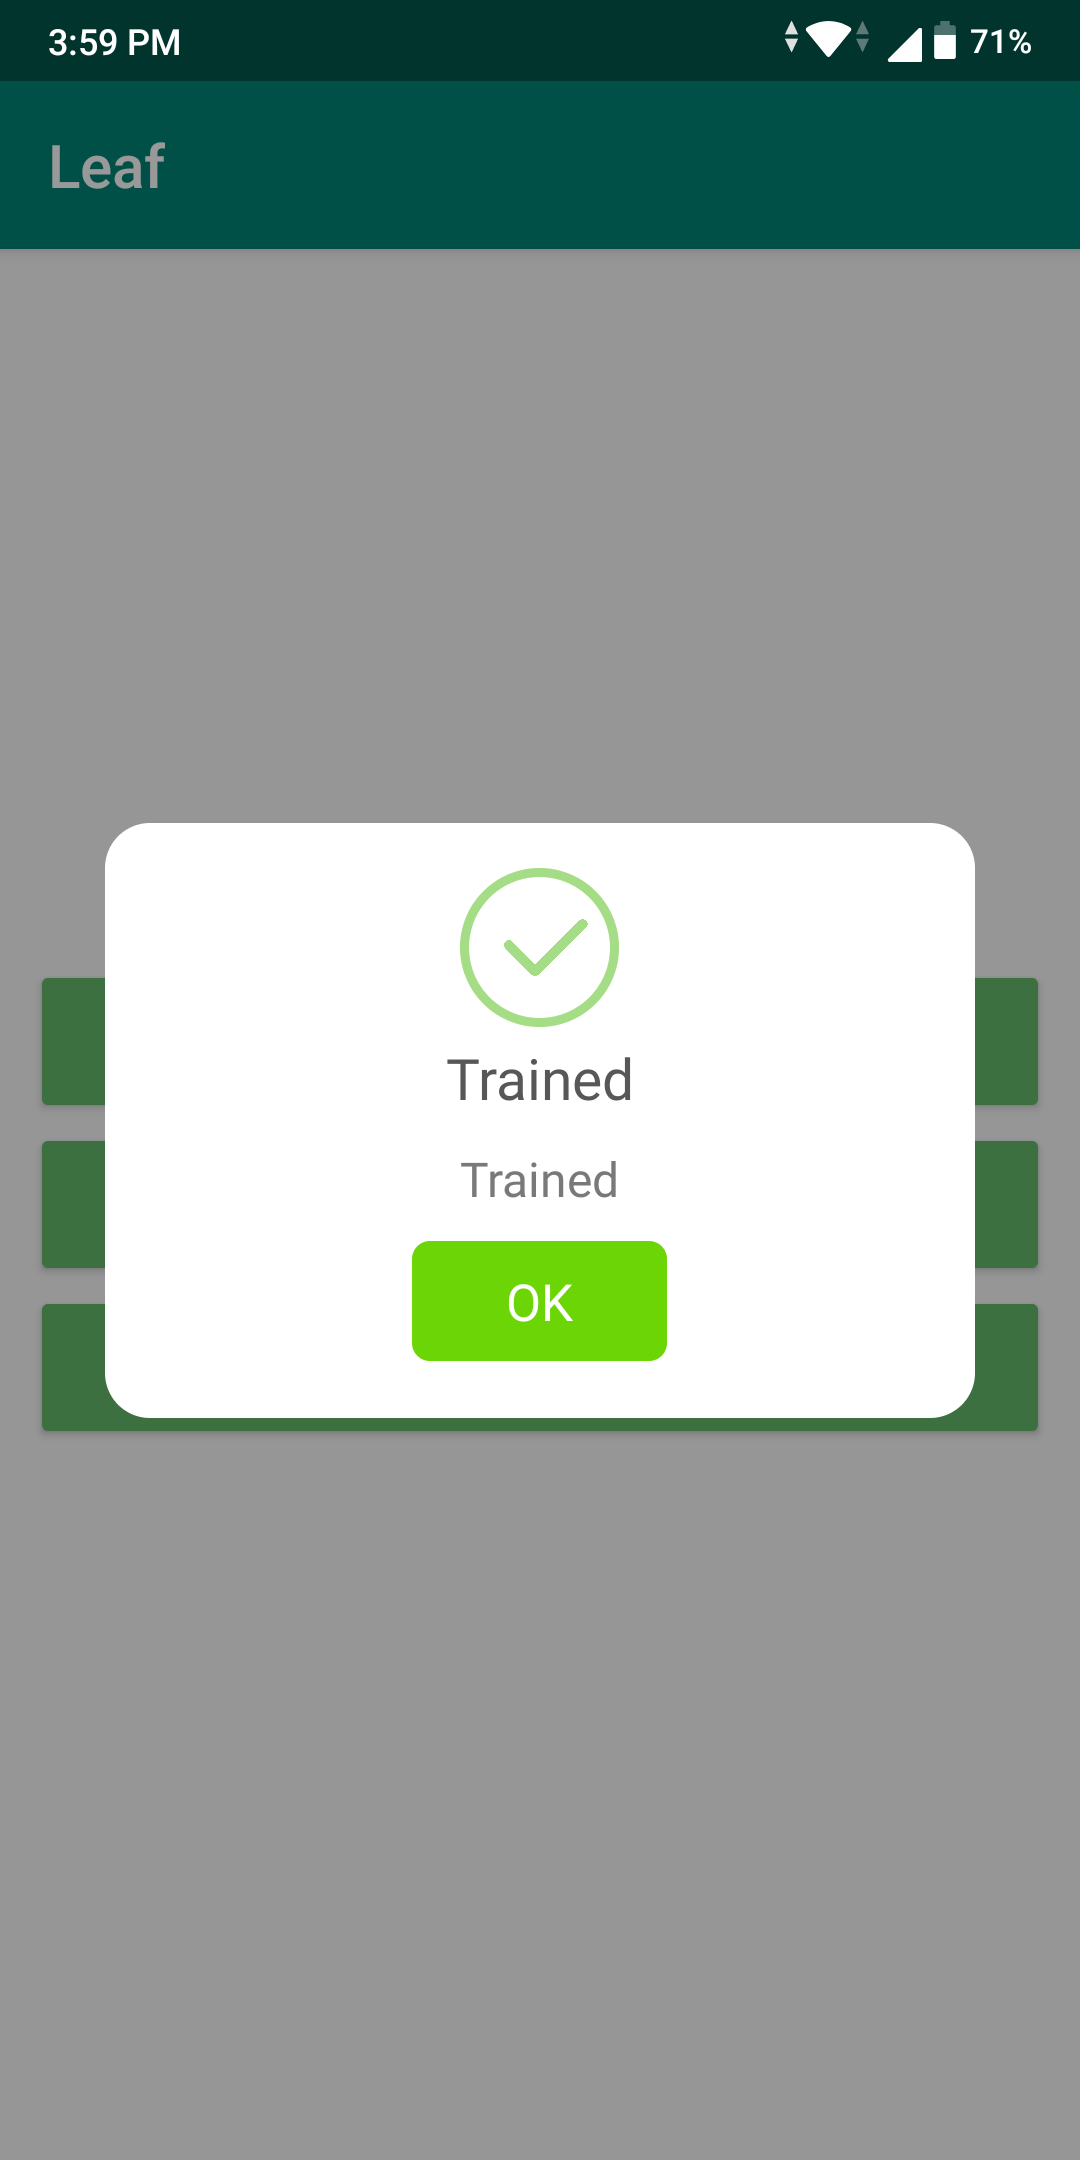
\includegraphics[width=0.5\textwidth]{bab5/figures/trained.png}
	\caption{Berhasil Train}
	\label{fig:train}
\end{figure}

\begin{figure}[ht]
	\begin{subfigure}{0.5\textwidth}
		\centering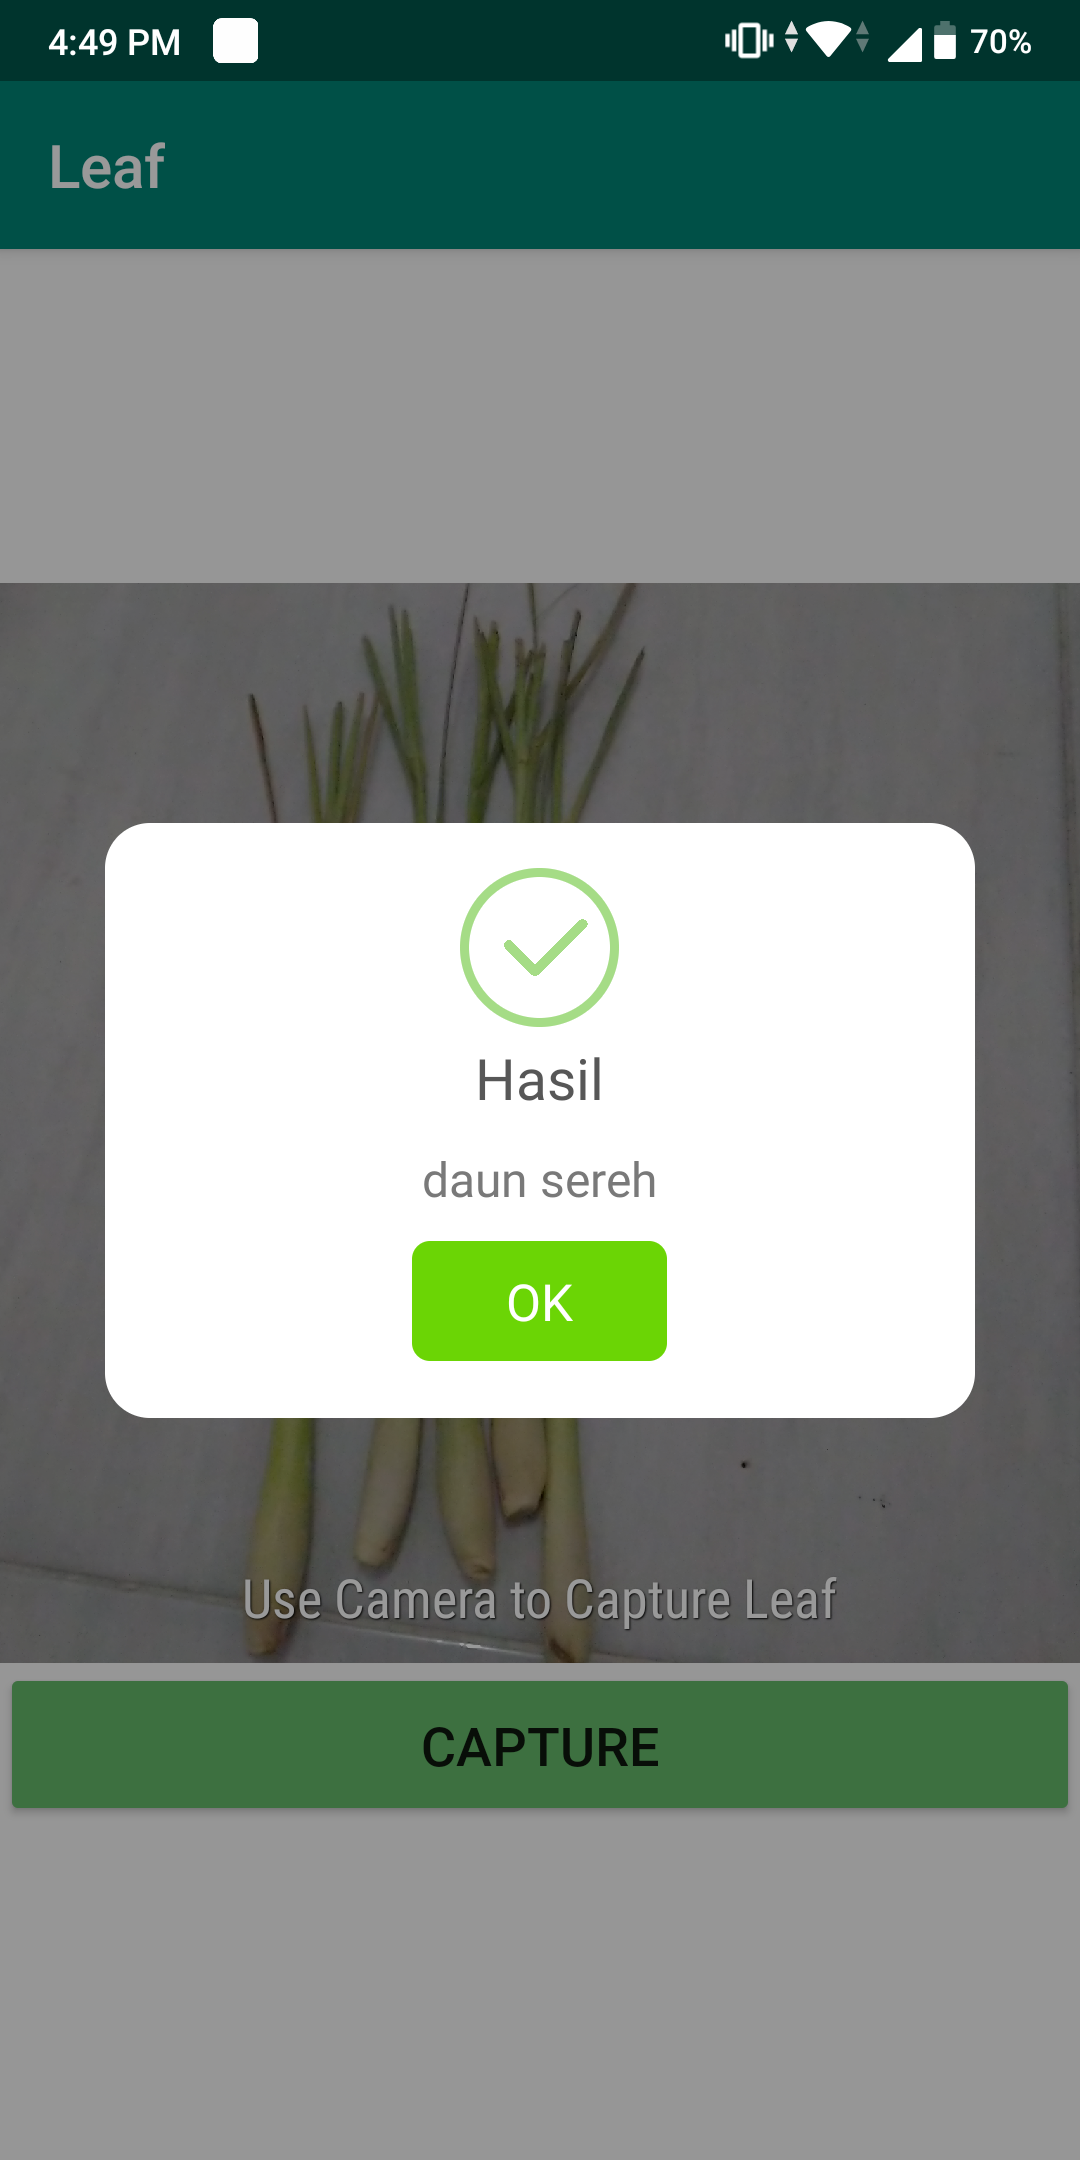
\includegraphics[width=\linewidth]{bab5/figures/ss2hasil.png}
		\caption{Hasil Prediksi Daun Sereh}
		\label{fig:hasil2}
	\end{subfigure}
	~
	\begin{subfigure}{0.5\textwidth}
		\centering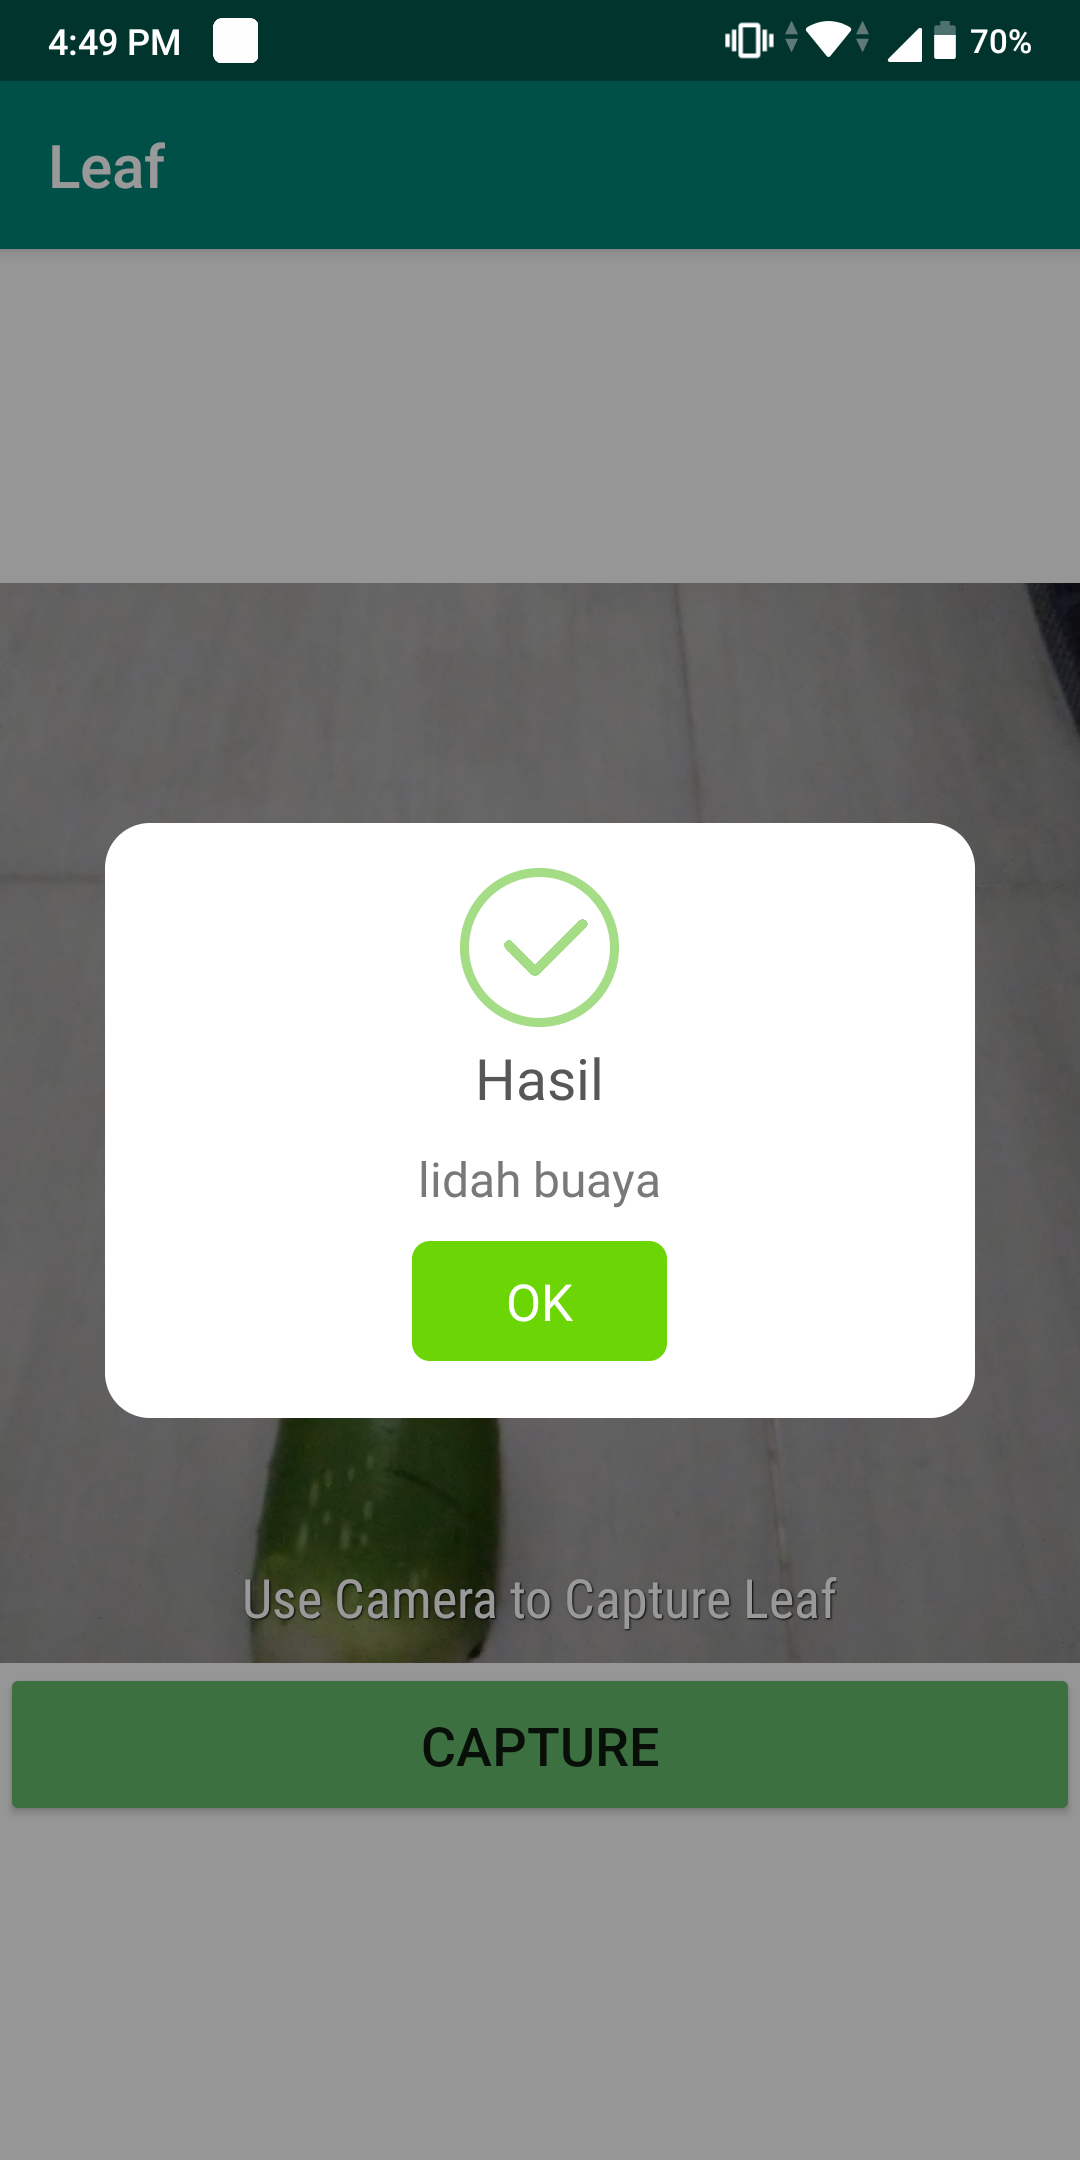
\includegraphics[width=\linewidth]{bab5/figures/ss1hasil.png}
		\caption{Hasil Prediksi Daun Lidah Buaya}
		\label{fig:hasil1}
	\end{subfigure}
\caption{Hasil tangkap layar pada fitur Predict}
\end{figure}

\begin{table}[ht]
	\centering
	\begin{tabularx}{1.0\textwidth}
		{|X|X|}
		\hline
		\rowcolor{lightgray} \centering Nama Daun& Hasil Benar dari 10 Pengujian\\ \hline
		\centering Lidah Buaya	& 	10 \\ \hline
		\centering Sereh	& 10  \\ \hline
		\centering Daun Jeruk	&	9 \\ \hline
		\centering Daun Beluntas	& 7	\\ \hline
	\end{tabularx}
	\caption{Tabel hasil pengujian pada daun}
	\label{table:hasil}
\end{table}


